\documentclass[tikz,border=10pt]{standalone}
\begin{document}
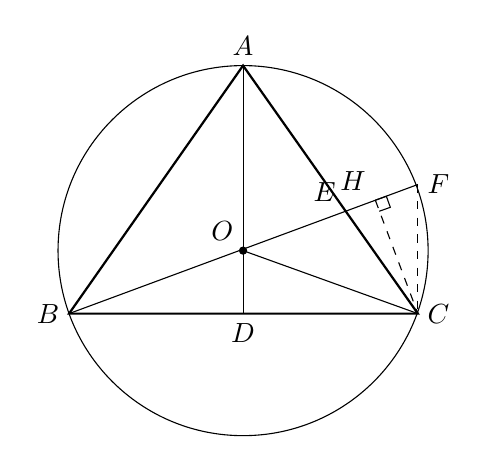
\begin{tikzpicture}
\coordinate (A) at (0,2.35);
\coordinate (B) at (-2.21,-0.80);
\coordinate (C) at (2.22,-0.80);
\coordinate (D) at (0,-0.80);
\coordinate (O) at (0,0);
\coordinate (E) at (1.30,0.50);
\coordinate (F) at (2.22,0.84);
\coordinate (H) at (1.68,0.64);

\draw (O) circle (2.35);

\draw[thick] (A) -- (B) -- (C) -- cycle;
\draw (A) -- (D);
\draw (B) -- (F);
\draw (O) -- (C);
\draw[dashed] (H) -- (C);
\draw[dashed] (F) -- (C);

\draw (1.68,0.64) -- (1.82,0.69) -- (1.87,0.55) -- (1.73,0.50);

\fill (O) circle (1.5pt);

\node[above] at (A) {$A$};
\node[left] at (B) {$B$};
\node[right] at (C) {$C$};
\node[below] at (D) {$D$};
\node[above left] at (O) {$O$};
\node[above left] at (E) {$E$};
\node[right] at (F) {$F$};
\node[above left] at (H) {$H$};
\end{tikzpicture}
\end{document}
